\documentclass[12pt]{article}
\usepackage{epsfig}
\usepackage{graphicx}
\usepackage{a4}
\usepackage{amsmath}
\usepackage{latexsym}
\usepackage{cite}
%\usepackage{draftwatermark}
\usepackage{lineno}
%\usepackage{chngcntr}
%\linenumbers


\usepackage{color}
\usepackage{colordvi}

\graphicspath{{Pics/}}
\DeclareGraphicsExtensions{.eps,.ps}

\textheight 22.0cm \textwidth 16.5cm
\oddsidemargin -0.1cm \evensidemargin -0.1cm

\usepackage{pslatex}
\usepackage[latin1]{inputenc}
\usepackage[T1]{fontenc}
\usepackage{amssymb}
\usepackage{url}

\newcommand{\msbar}{$\overline{\text{MS}}\, $}

%
% ----------------------------------------------------------------------------------------------
%
\begin{document}

\begin{titlepage}
\noindent
Draft 0.1  \hfill 05 June 2019\\
\\
DESY AA-BBB %\hfill  2019\\
\\

\vspace{1.3cm}

\begin{center}
  {\bf 

\large

Extraction of parton distribution functions using recent LHCb and ALICE heavy-flavour measurements
  }
  \vspace{1.5cm}

  {\large
    PROSA Collaboration
  }\\

  \vspace{1.2cm}

\end{center}
 %\input{authors.tex}  
  \vspace{2.4cm}
\begin{center}
\large
{\bf Abstract}
\vspace{-0.2cm}
\end{center}
%%
..............................
%%
\vfill
\end{titlepage}


%
% ----------------------------------------------------------------------------------------------
%
\newpage

\section{Introduction}
\label{sect:intro}

\section{Details of the QCD analysis}
\label{sec:qcdanalysis}
The QCD analysis consists of extraction input theoretical parameters (the PDF parameters and the quark masses) by minimising the $\chi^2$ between  data and theoretical predictions. 
It is performed using the xFitter framework~\cite{Alekhin:2014irh}. 
The $\chi^2$ minimisation is performed using the MINUIT package~\cite{James:1975dr} interfaced in xFitter.
The main objective of the QCD analysis is to constrain the gluon PDF in the proton at very low $x$ (up to $x \sim 10^{-6}$) by using measurements of charm hadroproduction. This provides a PDF set which can be reliably used in applications which require knowledge of the low-$x$ gluon, such as some astrophysical calculations~\cite{Garzelli:2015psa,Gauld:2015yia,Gauld:2015kvh,Garzelli:2016xmx,Bertone:2018dse} and MC underlying event tuning [any reference?].

\subsection{Input data}
\label{sec:data}

The following data sets are used in the present analysis:
\begin{itemize}
    \item combined Neutral Current (NC) and Charged Current (CC) inclusive DIS cross sections by H1 and ZEUS~\cite{Abramowicz:2015mha}
    \item combined charm and beauty NC DIS cross sections by H1 and ZEUS~\cite{H1:2018flt}
    \item measurements of charm hadroproduction by LHCb at 5 TeV~\cite{Aaij:2016jht}, 7 TeV~\cite{Aaij:2013mga} and 13 TeV~\cite{Aaij:2015bpa}, and by ALICE at 5 TeV~\cite{Acharya:2019mgn} and 7 TeV~\cite{Acharya:2017jgo}
    \item measurements of beauty hadroproduction by LHCb at 7 TeV~\cite{Aaij:2013noa}.
\end{itemize}
Compared to the previous PROSA analysis~\cite{Zenaiev:2015rfa}, this analysis uses more measurements of charm hadroproduction,\footnote{Since the main objective of the present analysis is to constrain the gluon PDF at low values of $x$ using the new LHC measurements of charm production, there was no intention to include other LHC measurements of beauty hadroproduction apart from those which were included in the previous analysis~\cite{Zenaiev:2015rfa}.}
as well as the final (and more precise) combined HERA data on inclusive NC and CC DIS, and heavy-quark production in NC DIS.

For the LHCb and ALICE data, the normalised cross sections as a function of rapidity, $\frac{{\rm d}\sigma}{{\rm d}y} / \frac{{\rm d}\sigma}{{\rm d}y_0}$, are calculated from the absolute cross sections and are used in the 
QCD analysis, with $\frac{{\rm d}\sigma}{{\rm d}y_0}$ being the cross section in the center bin, $3 < y < 3.5$, of 
the measured rapidity range in each $p_T$ bin (in particular, ALICE cross sections at $|y| < 0.5$ are normalised to LHCb cross sections at $3 < y < 3.5$). 
The advantage of using the normalised cross section, as was demonstrated in~\cite{Zenaiev:2015rfa}, is a significant
reduction of the scale dependence of the theoretical prediction, retaining the sensitivity of the cross sections to 
the PDFs. 

Bin-to-bin correlations in the input measurements are taken into account.
The treatment of correlated experimental uncertainties for the HERA data follows the original publications~\cite{Abramowicz:2015mha,H1:2018flt}.
For the ALICE and LHCb data, those correlated uncertainties which are reported as single numbers for all of $p_T$ and $y$ bins are treated as fully correlated, and uncorrelated uncertainties are obtained by subtracting the correlated ones from the total uncertainty. 
However, those systematic uncertainties which are reported as intervals are assumed to be uncorrelated, because the LHCb and ALICE publications do not provide information about their size in individual $p_T$ and $y$ bins. 
This missing information is mandatory for qualitative comparison to theoretical predictions (e.g.\ by means of the $\chi^2$ test) and future interpretation of precision measurements, and we encourage the LHC experiments to publish all eigenvectors of correlated uncertainties in individual bins (e.g.\ as the H1 and ZEUS experiments did in~\cite{Abramowicz:2015mha,H1:2018flt}).
In the QCD fit, for the normalised ALICE and LHCb cross sections the uncorrelated uncertainties on $\frac{{\rm d}\sigma}{{\rm d}y_0}$ are propagated as correlated uncertainties to the respective complementary rapidity bins. 

The $\chi^2$ definition follows that of Eq.~(32) in Ref.~\cite{Abramowicz:2015mha}.
For the heavy-quark normalised cross sections, the experimental uncertainties are treated as additive, and the treatment of the experimental uncertainties for the HERA DIS data follows the prescription given in Ref.~\cite{Abramowicz:2015mha}.

\subsection{Theoretical calculations}
\label{sec:th}

The analysis is performed at NLO (highest available order for heavy-quark hadroproduction) in the fixed-flavour-number scheme with three active flavours.
The PDFs are parametrised at the starting scale as described in Section~\ref{sec:pdfparam} and evolved to higher scales using the QCDNUM program~\cite{Botje:2010ay}.
Theoretical calculations for the HERA data sets are obtained using OPENQCDRAD~\cite{openqcdrad} following Ref.~\cite{H1:2018flt}.

Theoretical calculations for heavy-quark hadroproduction follow the previous PROSA analysis~\cite{Zenaiev:2015rfa}, with the only change is that we are using the \msbar mass scheme.
The predictions are computed using the MNR code for single-particle inclusive distributions in the pole mass scheme~\cite{Dowling:2013baa}, with the transition from the pole to the \msbar masses as described in~\cite{Dowling:2013baa}.
The factorisation and renormalisation scales are chosen to be $\mu_r = \mu_f = \sqrt{4m_Q(m_Q)^2+p_T^2}$, where $4m_Q(m_Q)$ is the \msbar heavy-quark mass. The heavy-quark masses are free parameters in the fit. 
The calculations are supplemented with phenomenological non-pertutbative fragmentation functions to describe the transition of heavy quarks into hadrons. 
As in the previous PROSA analysis~\cite{Zenaiev:2015rfa}, the fragmentation of charm quarks into D-mesons is described by the Kartvelishvili function with $\alpha_K = 4.4 \pm 1.7$ as measured at HERA~\cite{Aaron:2008ac,Chekanov:2008ur}, and for the fragmentation of beauty quarks $\alpha_K = 11 \pm 3$ is used as measured at LEP~\cite{Nason:1999zj}.

\subsection{PDF parametrisation}
\label{sec:pdfparam}

The gluon, valence quark and sea quark PDFs are parametrised at the starting scale $\mu^2_{f0} = 1.9$~GeV$^2$ of QCD evolution following Refs.~\cite{Abramowicz:2015mha}:
\begin{equation}\begin{aligned}
xg(x) &= A_{g} x^{B_{g}}\,(1-x)^{C_{g}}\, (1 + F_{g} {\log x}),\\
u_\mathrm{v}(x) &= A_{u_\mathrm{v}}x^{B_{u_\mathrm{v}}}\,(1-x)^{C_{u_\mathrm{v}}}\,(1+D_{u_\mathrm{v}}x) ,\\
d_\mathrm{v}(x) &= A_{d_\mathrm{v}}x^{B_{d_\mathrm{v}}}\,(1-x)^{C_{d_\mathrm{v}}},\\
x\overline{\mathrm{U}}(x)&= A_{\overline{\mathrm{U}}}x^{B_{\overline{\mathrm{U}}}}\, (1-x)^{C_{\overline{\mathrm{U}}}}\, (1+D_{\overline{\mathrm{U}}}x), \\
x\overline{\mathrm{D}}(x)&= A_{\overline{\mathrm{D}}}x^{B_{\overline{\mathrm{D}}}}\, (1-x)^{C_{\overline{\mathrm{D}}}}.
\end{aligned}
\label{eq:dv}
\end{equation}
Here $xg(x)$ is the gluon distribution, $xu_{\mathrm{v}}(x)$ and $xd_{\mathrm{v}}(x)$ are the up and down quark valence quark distributions, respectively, and $x\overline{\mathrm{U}}(x)$ and $x\overline{\mathrm{D}}(x)$ are 
the up- and down-type antiquark distributions, respectively, assuming relations $x\overline{\mathrm{U}}(x) = x\overline{u}(x)$ and $x\overline{\mathrm{D}}(x) = x\overline{d}(x) + x\overline{s}(x)$, with $x\overline{u}(x)$, $x\overline{d}(x)$, and $x\overline{s}(x)$ are the up, down, and strange antiquark distributions, respectively.
The sea quark distribution is defined as $x\Sigma(x)=x\overline{u}(x)+x\overline{d}(x)+x\overline{s}(x)$.
The normalisation parameters $A_{u_{\mathrm{v}}}$, $A_{d_\mathrm{v}}$, and $A_{g}$ are determined by the QCD sum rules.
The strangeness fraction $f_{s} = x\overline{s}/( x\overline{d} + x\overline{s})$ is fixed to
$f_{s}=0.4$ as in the HERAPDF2.0 analysis~\cite{Abramowicz:2015mha}.
Additional constraints $B_{\overline{\mathrm{U}}} = B_{\overline{\mathrm{D}}}$ and $A_{\overline{\mathrm{U}}} = A_{\overline{\mathrm{D}}}(1 - f_{s})$ are imposed to ensure the same normalisation for the $x\overline{u}$ and $x\overline{d}$ distributions as $x \to 0$.

The parameters in Eq.~(\ref{eq:dv}) are selected by first fitting with all parameters except $A$, $B$ and $C$ set to zero, and then including additional polynomial parameters one at a time until the $\chi^2$ of the fit is improved.
 The only exception is the $F_{g}$ parameter which does not improve the $\chi^2$ sizably (i.e.\ its fitted value is consistent with $0$ within uncertainty), but it affects the fit uncertainties significantly. The $F_g\log x$ term was proposed in~\cite{Bonvini:2019wxf} to provide a more flexible functional form at low $x$.
 
A special study was done to ensure the gluon PDF at low $x$ is not overconstrained: we parametrised the gluon distribution using functional forms from the ABMP16~\cite{Alekhin:2017kpj}, CT14~\cite{Dulat:2015mca}, HERAPDF2.0~\cite{Abramowicz:2015mha} and MMHT2014~\cite{Harland-Lang:2014zoa} PDF fits:
\begin{equation}
\begin{aligned}
\textrm{ABMP16:}~~~~~~ &xg(x)=A (1 - x)^b x^{a (1 + \gamma_{1} x)},\\
\textrm{CT14:}~~~~~~ &xg(x) = Ax^{a_1}(1-x)^{a_2}(e_0(1-y)^2+e_1(2y(1-y))+y^2), y=2\sqrt{x}-x,\\
\textrm{MMHT2014:}~~~~~~ &xg(x) = Ax^B(1-x)^C(1+a_1x+a_2(2x^2-1))+A^{\prime}_gx^{B^{\prime}_g}(1-x)^{25},\\ 
\textrm{HERAPDF2.0:}~~~~~~ &xg(x)=A_gx^{B_g}(1-x)^{C_g}+A^{\prime}_gx^{B^{\prime}_g}(1-x)^{25}.
\end{aligned}
\end{equation}
These functional forms are characterised by $4$ (ABMP16), $5$ (CT14, HERAPDF2.0) or $7$ (MMHT2014) parameters which control the gluon PDF (c.f.\ $4$ parameters in out nominal parametrisation in Eq.~\ref{eq:dv}). The fit using the HERAPDF2.0 and CT14 parametrisations yielded a gluon distribution with a sharp turnover to negative values at $x \sim 10^{-6}$, i.e.\ at the edge of the data sensitivity. As a result, such PDFs would predict a negative total charm hadroproduction cross sections at $\sqrt{s} \gtrsim 20$~TeV, as was already observed in~\cite{Garzelli:2015psa,Accardi:2016ndt}, therefore these parametrisations are discarded. The MMHT2014 parametrisation is similar to the HERAPDF2.0 parametrisation at low $x$, but the former is more flexible at high $x$. Our fit can not converge using the MMHT2014 parametrisation because there are not enough data to constrain the gluon PDF at high $x$, while discarding the extra parameters of the MMHT2014 parametrisation which control the high-$x$ gluon would result in the HERAPDF2.0 parametrisation. The ABMP16 parametrisation provides very similar results as our nominal parametrisation from Eq.~\ref{eq:dv}.

\subsection{Uncertainties}
\label{sec:pdfparam}

According to the general prescription used in the HERAPDF2.0 analysis~\cite{Abramowicz:2015mha}, 
the fit, model, and parametrisation uncertainties are taken into account.
Fit uncertainties are determined using the criterion of $\Delta\chi^2 = 1$ and the HESSE algorithm.
Model uncertainties are determined by varying the strangeness fraction $0.3 \leq f_{s} \leq 0.5$, the value of $Q^2_{\text{min}}$ imposed on the HERA data by $2.5 \leq Q^2_\textrm{min}\leq 5.0\textrm{GeV}^2$, the strong coupling constant by $0.105 < \alpha_s^{n_f=3}(M_Z) < 0.107$ (which corresponds to $0.117 < \alpha_s^{n_f=5}(M_Z) < 0.119$~\cite{Tanabashi:2018oca}), the fragmentation parameters $\alpha_K = 4.4 \pm 1.7$ for charm hadrons and $\alpha_K = 11 \pm 3$ for beauty hadrons, and the scales $\mu_f$ and $\mu_r$ for heavy quark production.
Originally the latter are varied up and down by a factor of two both simultaneously and independently for $\mu_r$ and $\mu_f$, however it was found that the simultaneous variation of $\mu_r$ and $\mu_f$ results in a larger PDF uncertainty in the bulk of the $x$ range. 
Therefore only the simultaneous $\mu_r$ and $\mu_f$ variation is used as a PDF uncertainty eigenvector.
The parametrisation uncertainty is estimated by extending the functional form in Eq.~(\ref{eq:dv}) with additional polynomial parameters, which are added or removed one at a time and do not improve the $\chi^2$. 
Also the gluon PDF is extended by adding the $+G_g\log^2 x$ term~\cite{Bonvini:2019wxf} (which does not improve the $\chi^2$ either; this term is not used in the nominal parametrisation, because the fit becomes unstable once even more additional parameters are introduced when determining parametrisation uncertainties).
Additionally, the parametrisation uncertainty is determined by varying $1.6 < \mu_\mathrm{f0}^2 < 2.2$~GeV$^2$.
The parametrisation uncertainty is constructed as an envelope, built from the maximal differences between the PDFs or QCD parameters resulting from the central fit and all parametrisation variations.
The total uncertainty is obtained by adding the fit, model, and parametrisation uncertainties in quadrature.

\section{Results}
\label{sec:results}

The fit yields a total $\chi^2 =2401$ for 1969 degrees of freedom, with partial $\chi^2$ of $1463$ and $938$ for the HERA and LHC data sets which have $1224$ and $760$ data points, respectively. The value
of $\chi^2$ per data point is about $1.2$ for both HERA and LHC data sets, and is similar in size to the value obtained in the analysis of the HERA combined inclusive data~\cite{Abramowicz:2015mha}. The global and partial $\chi^2$ values are listed in Table~\ref{tab:chi}. 
The central values of the fitted parameters with their fit uncertainties are given in Table~\ref{tab:pars}.

\begin{table}
\renewcommand*{\arraystretch}{1.12}
\tabcolsep1cm
    \centering
\begin{tabular}{ll}
    Dataset & $\chi^2/\textrm{ndp}$ \\
    \hline
    HERA1+2 CCep & 62 / 39  \\ 
    HERA1+2 CCem & 49 / 42  \\ 
    HERA1+2 NCem & 227 / 159  \\ 
    HERA1+2 NCep 820 & 68 / 70  \\ 
    HERA1+2 NCep 920 & 440 / 377  \\ 
    HERA1+2 NCep 460 & 223 / 204  \\ 
    HERA1+2 NCep 575 & 223 / 254  \\ 
    HERA c & 49 / 52  \\ 
    HERA b & 18 / 27  \\ 
    LHCb 7TeV [1302.2864] dzero nor. in y & 15 / 30  \\ 
    LHCb 7TeV [1302.2864] dch nor. in y & 19 / 29  \\ 
    LHCb 7TeV [1302.2864] ds nor. in y & 14 / 20  \\ 
    LHCb 7TeV [1302.2864] dstar nor. in y & 16 / 22  \\ 
    LHCb 7TeV Bzero pT-y cross section & 52 / 76  \\ 
    LHCb 7TeV Bch pT-y cross section & 129 / 108  \\ 
    LHCb 7TeV Bs pT-y cross section & 37 / 60  \\ 
    LHCb 5TeV [1610.02230] dzero nor. in y & 60 / 35  \\ 
    LHCb 5TeV [1610.02230] dch nor. in y & 25 / 35  \\ 
    LHCb 5TeV [1610.02230] ds nor. in y & 30 / 29  \\ 
    LHCb 5TeV [1610.02230] dstar nor. in y & 35 / 30  \\ 
    LHCb 13TeV [1510.01707] dzero nor. in y & 111 / 60  \\ 
    LHCb 13TeV [1510.01707] dch nor. in y & 72 / 64  \\ 
    LHCb 13TeV [1510.01707] ds nor. in y & 69 / 55  \\ 
    LHCb 13TeV [1510.01707] dstar nor. in y & 82 / 54  \\ 
    ALICE 7TeV [1702.00766] dzero nor. in y & 5.1 / 8  \\ 
    ALICE 7TeV [1702.00766] dch nor. in y & 0.75 / 7  \\ 
    ALICE 7TeV [1702.00766] dstar nor. in y & 2.3 / 6  \\ 
    ALICE 5TeV [1901.07979] dzero nor. in y & 6.3 / 10  \\ 
    ALICE 5TeV [1901.07979] dch nor. in y & 5.8 / 9  \\ 
    ALICE 5TeV [1901.07979] ds nor. in y & 2.5 / 4  \\ 
    ALICE 5TeV [1901.07979] dstar nor. in y & 1.7 / 9  \\ 
    \hline
    Correlated $\chi^2$  & 282  \\ 
    Log penalty $\chi^2$  &  -32  \\ 
    \hline
    %\rowcolor{white}
    %\midrule
    Total $\chi^2$ / dof  & 2401 / 1969  \\ 
    %\rowcolor{white}
    %\midrule
    %$\chi^2$ p-value  & 0.00 & 0.00   \\ 
    %\bottomrule
\end{tabular}
\caption{The global and partial $\chi^2$ values for each data set together with the corresponding number of data points (ndp). The correlated $\chi^2$ and the log penalty $\chi^2$ entries refer to the $\chi^2$ contributions from the correlated uncertainties and from the logarithmic term, respectively, as described in Ref.~\cite{Abramowicz:2015mha}.}
\label{tab:chi}
\end{table}

\begin{table}
    \renewcommand*{\arraystretch}{1.12}
    \tabcolsep1cm
    \centering
\begin{tabular}{ll}
    Parameter & Value \\
    \hline
    $B_g$ & $0.004 \pm 0.053$  \\
    $C_g$ & $6.25 \pm 0.29$  \\
    $Fg$ & $0.068 \pm 0.024$  \\
    $B_{u_v}$ & $0.644 \pm 0.030$  \\
    $C_{u_v}$ & $4.862 \pm 0.076$  \\
    $E_{u_v}$ & $15.8 \pm 2.2$  \\
    $B_{d_v}$ & $0.873 \pm 0.076$  \\
    $C_{d_v}$ & $4.61 \pm 0.35$  \\
    $C_{\overline{U}}$ & $7.36 \pm 0.77$  \\
    $D_{\overline{U}}$ & $10.1 \pm 2.4$  \\
    $A_{\overline{D}}$ & $0.1061 \pm 0.0058$  \\
    $B_{\overline{D}}$ & $-0.1661 \pm 0.0062$  \\
    $C_{\overline{D}}$ & $12.7 \pm 3.0$  \\
    $m_c(m_c)$ & $1.230 \pm 0.031$ GeV  \\
    $m_b(m_b)$ & $3.977 \pm 0.100$ GeV  \\
\end{tabular}
\caption{The fitted parameters with their fit uncertainties.}
\label{tab:pars}
\end{table}

The fitted PDFs with their total uncertainties at the scale $\mu^2_f=10$ GeV$^2$ are shown in Fig.~\ref{fig:pdfs}. They are superimposed with the PDFs from the PROSA 2015 fit~\cite{Zenaiev:2015rfa}. Furtheromore, Fig.~\ref{fig:pdfratios} (left) displays the gluon distribution normalised to the one from the PROSA 2015 fit. 
A significant reduction of the gluon PDF uncertainty is achieved at $x < 10^{-4}$ compared to the PROSA 2015 fit. 
The results of the two fits for the gluon PDF are in good agreement: the central value from the new fit is always within the PROSA 2015 uncertainty band. 
The changes of the valence and sea quark distributions are attributed to the replacement of the HERA-I DIS data which were used in the PROSA 2015 fit with the new combined final HERA data and are consistent with the HERAPDF2.0 analysis~\cite{Abramowicz:2015mha}: the shape of the valence distributions is harder, while the sea distribution of the new fit at high x is softer. 
To check further the new PDFs, we have calculated prediction for H1, ZEUS and CMS measurements of jet production, and CMS measurement of $t\bar{t}$ production which are implemented in xFitter using our VFNS fit (see Appendix), and found the new PDFs describe all these data sets better than the predictions obtained using HERAPDF2.0.

The relative total, fit, model and parametrisation uncertainties for the gluon PDF are shown in Fig.~\ref{fig:pdfratios} (right). The total uncertainties are dominated by the model uncertainties, with the largest contributions to the latter given by the scale variations for heavy-quark hadroproduction. Higher order calculations are needed to reduce these uncertainties.

The resulting PDFs are available in the LHAPDF format at [\dots].
In addition, we perform a fit using a variable-flavour-number scheme (VFNS), described in Appendix. These PDFs might be useful for MC underlying event tuning.

\begin{figure}
    \centering
    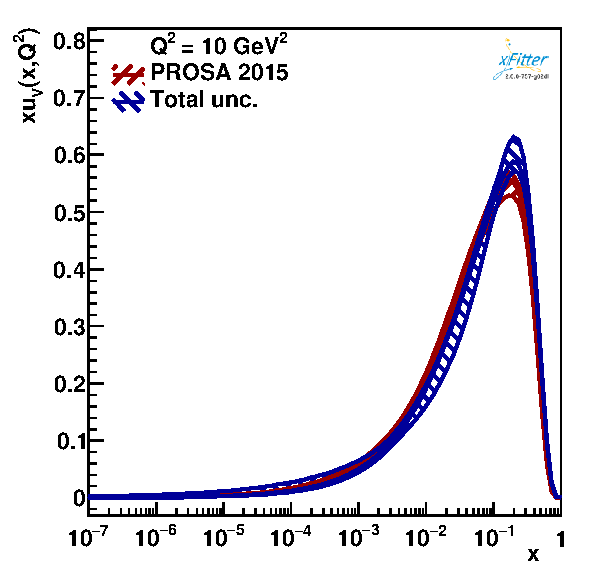
\includegraphics[width=0.49\textwidth]{figs/q2_10_pdf_uv.pdf}
    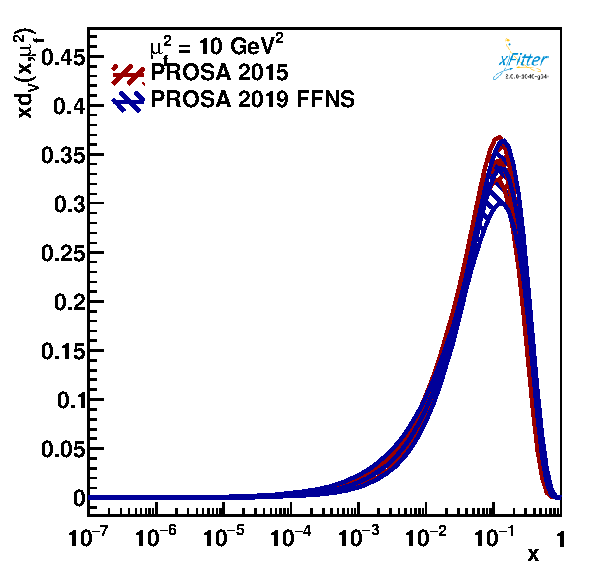
\includegraphics[width=0.49\textwidth]{figs/q2_10_pdf_dv.pdf}\\
    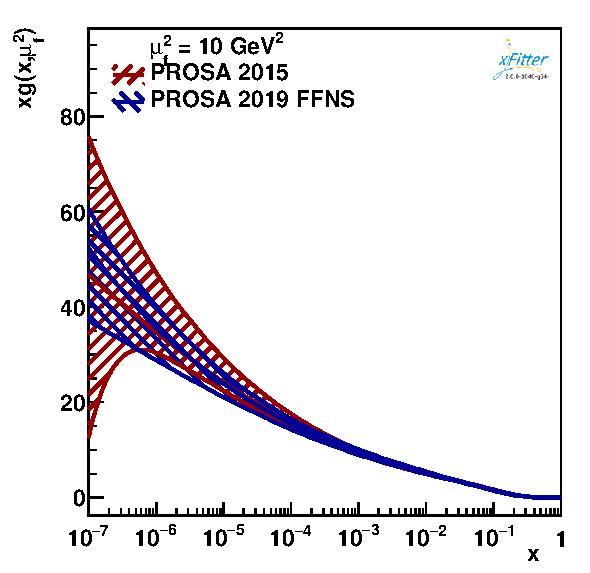
\includegraphics[width=0.49\textwidth]{figs/q2_10_pdf_g.pdf}
    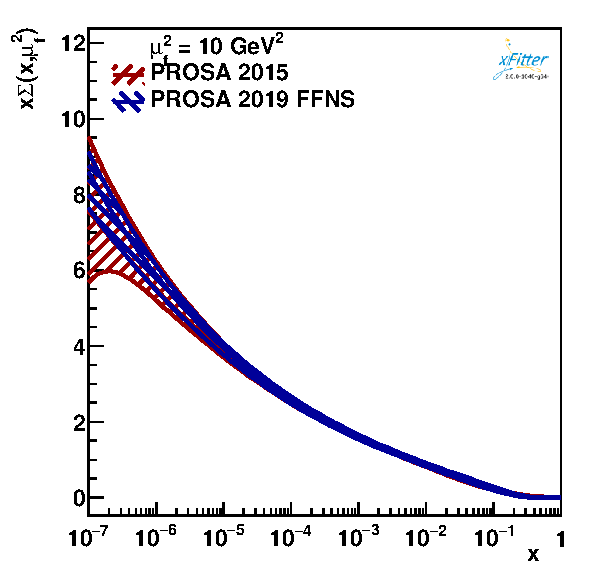
\includegraphics[width=0.49\textwidth]{figs/q2_10_pdf_Sea.pdf}
    \caption{The fitted PDFs with their total uncertainties at the scale $\mu^2_f=10$ GeV$^2$ compared with the distributions form the PROSA 2015 fit.}
    \label{fig:pdfs}
\end{figure}

\begin{figure}
    \centering
    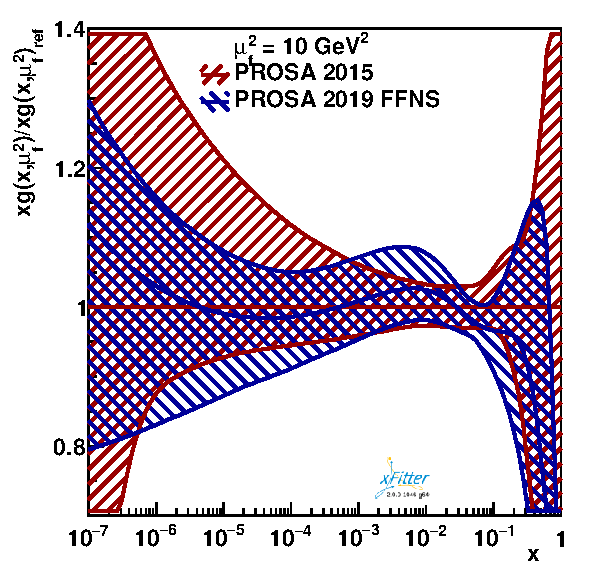
\includegraphics[width=0.49\textwidth]{figs/q2_10_pdf_g_ratio.pdf}
    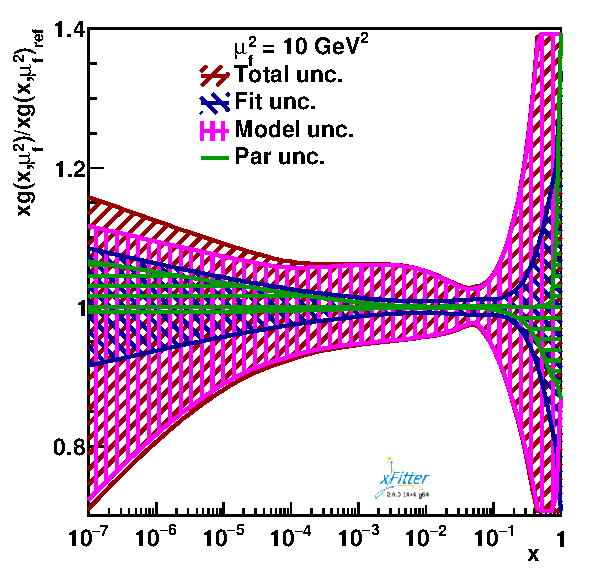
\includegraphics[width=0.49\textwidth]{figs/gluonunc.pdf}
    \caption{(left) The gluon PDF with their total uncertainties at the scale $\mu^2_f=10$ GeV$^2$ divided by the gluon PDF from the PROSA 2015 fit. (right) The relative total, fit, model and parametrisation uncertainties for the gluon PDF at the scale $\mu^2_f=10$ GeV$^2$.}
    \label{fig:pdfratios}
\end{figure}

\subsection{Astrophysical application}
\label{sec:astro}

\section{Summary}
\label{sec:summary}

\section*{Acknowledgements}

%  We would like to thank ...
The work of O.~Z. has been supported by Bundesministerium f\"ur Bildung und Forschung (contract 05H18GUCC1).

%%%%%%%%%%%%%%%%%%%%%%%%%%%%%%%%%%%%%%%%%
%%%%%%%%%%%%%%%%%%%%%%%%%%%%%%%%%%%%%%%%%

\bibliographystyle{unsrt}
\bibliography{prosa2019,extra}

\clearpage
\appendix
\section{Fit in VFNS}
\label{sec:vfns}

The fit in the VFNS is performed using the APFEL library~\cite{Bertone:2013vaa} interfaced in xFitter.
The theoretical predictions for the HERA data are computed using the FONLL-B scheme~\cite{Forte:2010ta} with the pole charm and beauty quark masses set to $m_c^{\textrm{pole}} = 1.4$ GeV and $m_c^{\textrm{pole}} = 4.5$ GeV respectively.
However, no VFNS calculation for heavy-quark hadroproduction is available publicly in the format which can be used for PDF fitting.
To keep using the MNR calculations with the VFNS, we exploit the feature of the APFEL library to choose arbitrary heavy-quark matching thresholds~\cite{Bertone:2017ehk}. These thresholds are set to values:
\begin{equation}
\begin{aligned}
\mu_c &= 4.5m_c^{\textrm{pole}} = 6.3~\textrm{GeV},\\
\mu_b &= 4.5m_b^{\textrm{pole}} =  20.25~\textrm{GeV}.
\end{aligned}
\end{equation}
We imposed kinematic cuts $p_T < 5$ GeV and $p_T < 16$ GeV on the LHC charm and beauty data, respectively, to ensure that we are working with not more than 3 (4) flavours when calculating predictions for charm (beauty) data. The strong coupling strength is set to $\alpha_s^{n_f = 5}(M_Z) = 0.118$~\cite{Tanabashi:2018oca}, while all other settings are the same as in the FFNS fit.
The choice of the matching thresholds is arbitrary and amounts to a renormalisation scheme choice~\cite{Bertone:2017ehk}, therefore we have verified that the fit results are stable under variations within $3.1 \le \mu_Q/m_Q^{\textrm{pole}} \le 6$, with the $p_T$ cuts on the charm and beauty LHC data modified accordingly.

The resulting PDFs are available in the LHAPDF format at [\dots]. No PDF uncertainties are provided with this set.




\end{document}


